\documentclass[12pt]{article}
\usepackage{latexsym}
\usepackage{caption2}
\usepackage{flafter}
\usepackage{graphicx}
\usepackage[sort,numbers]{natbib}
\setlength{\bibsep}{-0.5pt}
\usepackage{tcolorbox}
\newtcolorbox{mybox}{colback=grey!5!white,colframe=red!75!black}
\usepackage[]{setspace}
\usepackage{amsfonts}
\usepackage{amssymb,amsmath}
%\usepackage[table]{xcolor}
\usepackage[mathlines,displaymath]{lineno}
\usepackage[T1]{fontenc}
\usepackage[latin1]{inputenc}
\usepackage{anyfontsize}
\usepackage{lipsum}
\usepackage{etoolbox}
\usepackage{float}
\usepackage{wrapfig}
\makeatletter
\patchcmd{\@maketitle}{\begin{center}}{\begin{flushleft}}{}{}
\patchcmd{\@maketitle}{\begin{tabular}[t]{c}}{\begin{tabular}[t]{@{}l}}{}{}
\patchcmd{\@maketitle}{\end{center}}{\end{flushleft}}{}{}
\makeatother

\newcommand{\etal}{{et~al.{}}}
\newcommand{\ie}{{i.~e.{}}}
\newcommand{\eg}{{e.~g.{}}}
\newcommand{\viz}{{viz.{}}}
\newcommand{\etc}{{etc.{}}}
\newcommand{\apriori}{{a priori{}}}
\newcommand{\vv}{{vice versa{}}}
\newcommand{\cf}{{}}
\usepackage{titling}
\usepackage{color}
\newcommand{\carlos}[1]{\textcolor{red}{#1}}
\newcommand{\toedit}[1]{\textcolor{blue}{#1}}
\setlength{\droptitle}{-10em}% This is my set screw

\oddsidemargin 0.35cm 
\textwidth 17cm 
\textheight 20.75cm 

\begin{document}
\pagestyle{empty}

\section*{Part 2: Description of Work}

\section*{1. Summary}
<<<<<<< HEAD
Biological systems consist of elements that interact within and across
levels. For example, interactions among genes and plasticity determine
traits of individuals and adaptations to environments and habitats,
competitive and cooperative interactions among individuals influence
population dynamics, and interactions among species affect the
dynamics of communities and ecosystem processes. Such systems,
classically studied as simple graphs, can be explored as networks of
networks to capture the interactions inside and between networks,
interdependencies among hierarchical levels, and in general, the
connectivity patterns and processes across the different scales of
biological organization (Figure 1).

{\bf BIODIVERSITY DYNAMICS 
 
BIODIVERSITY DECLINE 

DIVERSIFICATION}

=======
Biological systems consist of elements that interact within and across levels. For example, interactions among genes and plasticity determine traits of individuals and adaptations to environments and habitats, competitive and cooperative interactions among individuals influence population dynamics, and interactions among species affect the dynamics of communities and ecosystem processes. Such systems, classically studied as simple graphs, can be explored as networks of networks to capture the interactions inside and between networks, interdependencies among hierarchical levels, and in general, the connectivity patterns and processes across the different scales of biological organization (Figure 1).
>>>>>>> 9bd86e7a971d845b186e97178ddabf79dab974a8
\\
Statements of the goals

We propose to study interactions within and between biological levels to decipher key interdependencies that maintain biodiversity in ecosystems. We bridge data science and theories of biodiversity on the shoulders of recent studies focusing on the entangled web of life, that is, interactions and interdependencies across genetic, phenotypic, ecological and spatial scales, represented each data set as a network. Our goal is to test the need to disentangle a multilayer network to understand biodiversity, that is, a simple graph approach is not enough to understand biodiversity. The understanding of the webs of life requires the entanglement of several layers of data-driven theory.
\\
Milestones

i) Data animations
To developing visualizations of genetic, phenotypic, ecological and spatial data to 1) Gain insights on how the the interactions connecting inside and across biological levels drive the evolution and maintenance of biodiversity, and 2) Communicate in public exhibitions the core patterns and processes governing interdependent networks across biological levels.
\\
ii) Data mining and NoN inference. To infer patterns of interdependence within and between genetic, phenotypic, ecological, and spatial networks {\bf THIS IS REPETITIVE to gain insights into the connectivity within and across biological levels} (Box 1).
\\
iii) iii)	Processes driving tangled webs. To Infer mechanisms using data-driven modeling scenarios coupling genetic, phenotypic, ecological, and spatial networks {\bf THIS IS REPETITIVE to explore how connectivity patterns within and between levels alter biodiversity patterns} (Box 2).
\\
Significance of the project for data science

The increase in availability of biological data and computational power together with new
methods presents many opportunities to strengthen the interplay between ecological and
evolutionary processes maintaining diversity. Yet, while data science is progressing in merging
patterns and processes for the existing large-scale data in many fields, the integration of
patterns and processes integrating data across biological levels in ecology and evolution is still
at a very incipient stage. In this project we envision three main advances for data science:
i) Strengthening the feedback between data science and data-driven synthesis in ecology and
evolution. We will release a data-driven package scalable to other datasets to decipher the
strength of interdependencies across biological networks, the patterns and mechanisms that
underlie such interdependencies and their effects on biodiversity maintenance, and
ii) Communicating throughout animations in a permanent public exhibition the importance of
using interdependent biological networks in merging data science, ecological and evolutionary
processes for the maintenance of biodiversity.


\section*{2. Background}

The study of interactions, both within and across hierarchical scales,
is central to the ongoing synthesis of ecology and evolution in
general \citep{Darwin:1964,Futuyma&Slatkin:1983,Thompson:2013}, and to
debates surrounding the relationship between complexity and stability
in particular. Ecologists, for example, have argued for empirical
patterns of positive \citep{MacArthur:1955}, negative \citep{May:1973}
and non-relationships \citep{Jacquetetal:2016} between the number of
links and the stability of food webs (i.e., the number of links
usually defined as the complexity of the food web). This debate is
rooted in the mechanisms driving ecological interactions within and
among species
\citep{May:1973,dunne2005modeling,Thebault&Fontaine:2010,Allesina&Tang:2012,Johnsonetal:2014,Mougi&Kondoh:2016,Graveletal:2016}. Analogously,
evolutionary biologists have puzzled over the relationships between
the complexity of gene interactions and the stability of phenotypes
\citep{Alberch:1991,Arnold:1992,Debat&David:2001,Wagner:2005}. Quantitative
genetics theory predicts that most genetic variance in populations is
additive \citep{Hilletal:2008}, and yet accounting for gene
interactions can improve predictions about the distribution and
evolution of traits \citep{Forsbergetal:2017}. Experiments are also
increasingly showing that gene interactions are common and that
additivity can be an emergent property of underlying genetic
interaction networks
\citep{Stearns:2010,EyreWalker:2010,Wagner&Zhang:2011,Mackay:2014,North&Beaumont:2015,Pavlicevetal:2015}.

Although the relationship between complexity and stability has been
explored within hierarchical levels, such as either individuals,
populations or food webs, the relationship among levels has received
less attention
\citep{Whithametal:2006,Loeuille:2010,Fontaineetal:2011}. Eco-evolutionary
theory usually includes interactions in one hierarchical level
network, therefore we do not have a good understanding of how to
integrate data and theory to connect complex traits to the stability
and complexity of ecological networks. It is possible that small-scale
interactions at one hierarchical level might help explain large-scale
patterns at another (``Hierachical networks'' in Figure 1). For
example, networks of gene interactions and migration dynamics could plausibly influence
trait-dependent interactions between populations. In such hierarchical
systems, what is the relationship between complexity and stability?
<<<<<<< HEAD
\begin{center}
\hspace{-2 in}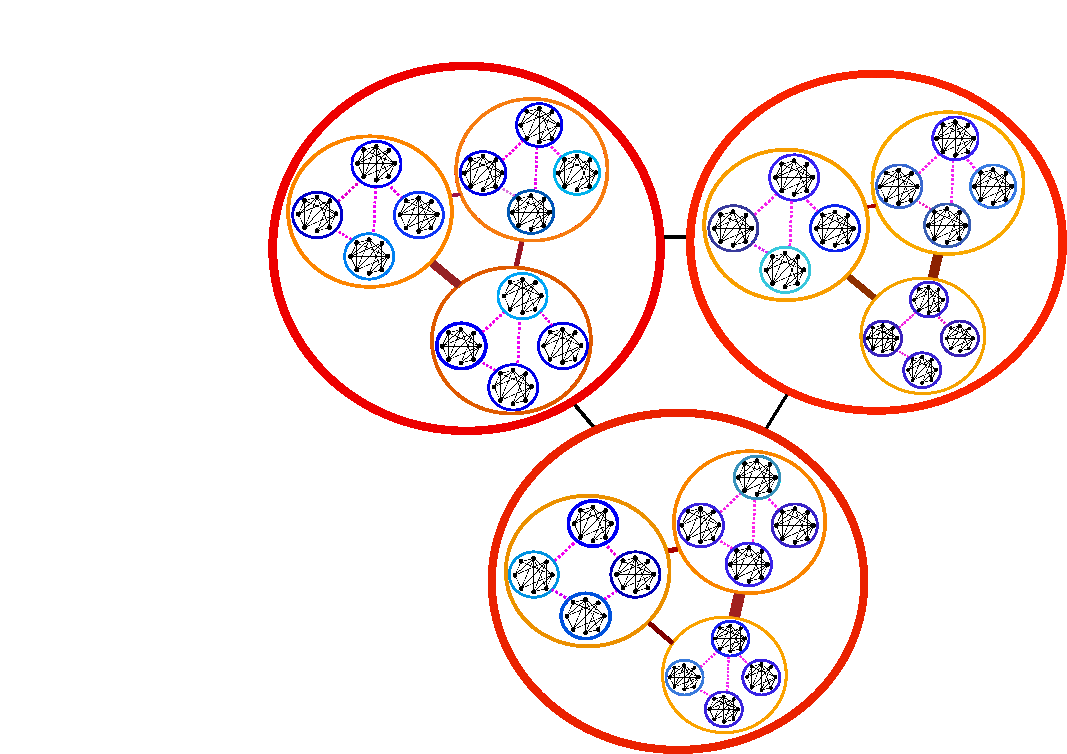
\includegraphics[width=17cm,height=13cm]{Figure1.pdf}
\\
=======

%\vspace{-1 in}
\begin{center}
\hspace{-2 in}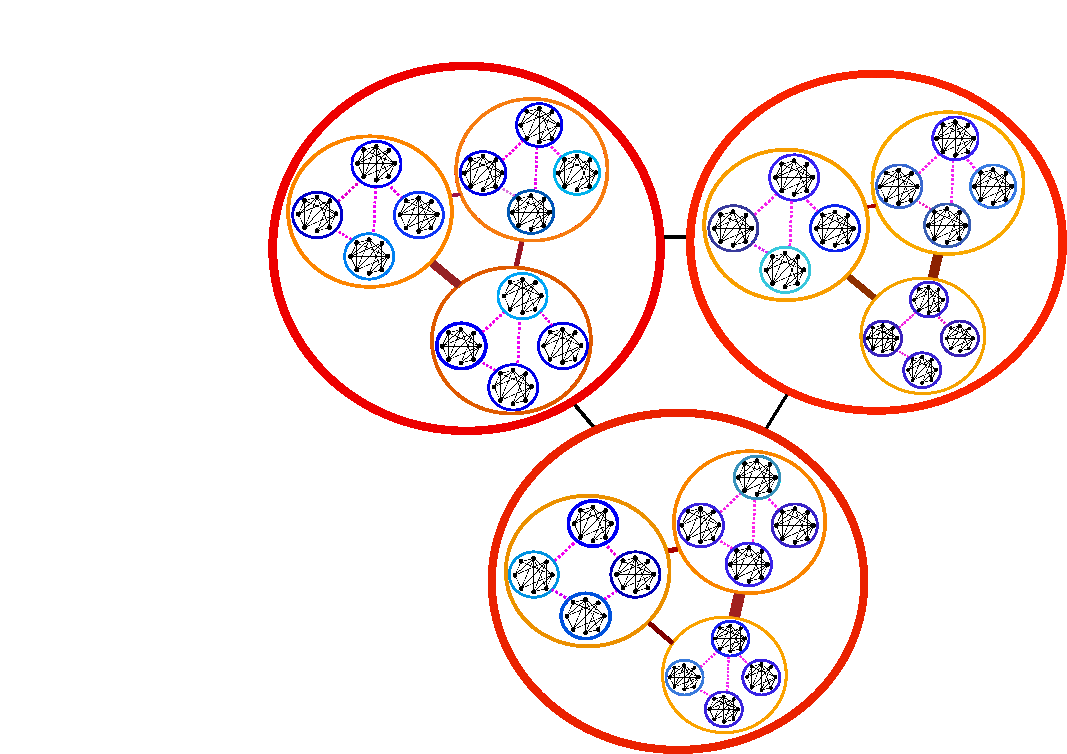
\includegraphics[width=17cm,height=13cm]{Figure1.pdf}
>>>>>>> 9bd86e7a971d845b186e97178ddabf79dab974a8
\caption{{\small Figure 1: Hierarchical network approach: We represent a meta-ecosystem
  with patches (red), species (orange), individuals (blue), and genes
  (black). At intra-organismal level, genes interact to produce a
  trait (blue). At inter-organismal level individuals mate (dotted
  pink links) to produce the distribution of traits (blue tones). At
  population level trait distribution drives the interaction strength
  between species (brown links). The meta-ecosystem is pictured as a
  spatial network (black links) of local interaction networks.}}
\vspace{2 in}
\label{Figure 1}
\end{center}
<<<<<<< HEAD
\vspace{-1 in}
=======
\vspace{-4 in}
>>>>>>> 9bd86e7a971d845b186e97178ddabf79dab974a8

\section*{3. Significance to Data Science, Scientific Goals and Objectives}

Data spanning many branches of ecology and evolution are starting to
decipher the interaction patterns across levels of biological
organization and the relationship between complexity and stability
\citep{Kivelaetal:2014,Ahnetal:2010,DeDomenico:2014,Morrison&Badyaev:2016}. Many
libraries are also rapidly emerging to integrate, analyze and
visualize patterns across networks
\citep{Schneideretal:2011,Kivela:2013,DeDomenico:2014,Kivelaetal:2014}. For
example, recent analysis of six different levels of biological
organization depicting gene interactions, complex phenotypes, animal
societies, metapopulations, food webs, and vertebrate communities has
shown invariant patterns of nestedness independently of the
interaction type or biological scale \citep{Cantoretal:2017}. In a
nested network interactions are organized such that specialists (for
example predators that eat only a few prey) interact with a subset of
the species with whom generalist, for example, predators that attack
many preys, interact. Nestedness has received significant attention
because it has been suggested that a nested pattern of interactions
may lead to greater or lower biodiversity in ecological networks
\citep{Bastollaetal:2009,Staniczenkoetal:2013}. Regardless of whether
nestedness or other network pattern increase or decrease the number of
species in ecological networks, it is an open question how data-driven
inference methods can help to capture the interdependencies in
hierarchical networks and which ecological and evolutionary processes
drive such interdependency. Therefore, our the goals of this proposal are:
\begin{itemize}
\item Combine visualization and animations to exploratory analysis and
  computaton of metrics to detect network patterns crossing two or
  more networks using our source data hosted by $Renga$ $Platform$.
\item Team up with the SDSC staff the implementation of Markov random
  field methods to efficiently compute and/or reconstruct the
  interdependencies among genetic, phenotypic, ecological and spatial
  networks (Box 1).
\item Implementing, debugging, and analyzing meta-ecosystem
  eco-evolutionary network process-based modeling scenarios
  parametrized using the inference patterns obtained in goal 2 (Box
  2). This step will use linear algebra techniques to contrast the
  stability-diversity properties of multilayer networks between
  scenarios driven by the empirical patterns and theoretical scenarios
  using null or neutral models.
\end{itemize}

\section*{4. Research Plan}

\section*{4.1 General description of the scientific approach}

<<<<<<< HEAD
We describe our scientific approach in Box 1 highlighting 1) the integration between data-driven and process-based approaches in biodiversity research, 2) the existing model systems to understand the multilayer nature of biodiversity, and 3) a modeling prototype bridging data-driven and process-based approaches connecting multilayer networks with deep learning networks. 

Biodiversity research has been systematically studied at only one biological level and splitted in many temporal and spatial scales. This has produced an immense gain in detailed knowledge at each of the levels and scales studied, but the one-level and one-scale approach might be insufficient to understand diversification, biodiversity dynamics and biodiversity decline under human-driven disturbances. For example, we might think that the decline of one species is due to low genetic diversity in response to a rapidly changing environment. However, this decline can be triggered by the absence or the presence of specialized predators-parasites in specific habitats and\or by the genetic architecture of the complex traits involved in the prey-predator-parasites interactions. Taking together, to understand the decline of one species we would need not only the genetic variance, but also the community of predators-parasites and the architecture of the defense traits across the landscape. On the other hand, there are a few model systems where multidimensional individual data have been collected (See section 4.2 Data Sources, Figure 2) but datasets collected at multiple levels or scales are currently missing. This situation leaves us in a data and methods gap meaning we currently do not have datasets collected or integrating different biological levels and spatial scales to be confronted against deep process-based learning networks framing different scenarios of connections within and among layers \citep{Reichsteinetal:2019}. 
 

\begin{mybox}\begin{singlespace}
{\bf{Box 1. Deep learning and multilayer networks in Biodiversity research}}\\
\begin{small} 
 Our approach will contain two steps. First, we will join data-driven inference with process-based approaches to decipher the mechanisms that best predict the patterns within and among the layers of collected data (section 4.2 Data Sources.) Second, we will run deep process-based learning models exploring a broad range of biodiversity datasets to explore the network configurations within and between layers that maintain biodiversity.\\
  {\small Step 1: Deep learning networks in biodiversity data}}
  We will explore networks with varying structures to infer the ones minimizing the difference with the empirical patterns DESCRIPTION OF EMPIRICAL PATTERNS. The starting point will be to explore networks allowing for feedbacks and nonlinear functions within and between layers (Figure 2). WHY THESE NETWORKS We will explore a range of topologies from bidirectional recurrent neural networks (BRNN) to feedforward neural networks (FNN) and reinforcement learning in unknown environments (RL) \citep{Schmidhuber:2015}.\\
  {\small Inference}
  Most data sets in ecology and evolution are large collections of small data sets (See section 4.2 Data Sources.) For example, in areas such as species ranges and species interactions, there might be a large amount of data, but there is still a relatively small amount of data for each gene, phenotype, individual or interaction. To customize predictions for species ranges and accounting for abiotic and biotic factors it becomes necessary to build scenarios accounting for the heterogeneity at individual level, with its inherent uncertainties, and to couple these models together in a hierarchy scaling from genes, to phenotypes, populations, communities and ecosystems, so that information can be borrowed from other similar levels across the landscape in the absence of empirical estimations. This individualization of models \citep{Ghahramani:2015}, will be implemented using hierarchical Bayesian neural networks approaches such as hierarchical Dirichlet processes therefore accounting for many interdependent layers.\\
  {\small Step 2: Deep process-based learning networks in biodiversity research}
  We will explore a suite of deep process-based learning networks to infer the role of feedbacks between evolutionary and ecological networks on biodiversity dynamics. We will account for demography, trait evolution, gene flow and selection regimes across many interacting species across landscape gradients (Box 2). We will integrate datasets from many taxa to decipher the most plausible network configurations within and between layers that maintain biodiversity (https://github.com/melian009/Robhoot/blob/master/layers/data.integration/databases.md). Box 2 describes the starting point to explore further additional network topologies considering BRNN, FNN and RL type networks. We will explore how disturbance affect biodiversity loss in two different scenarios (i.e., independent layers and feedbacks). As a consequence of this exploration, we aim to advance which data will be needed to collect or integrate at different levels and scales to better understand biodiversity dynamics. Which mechanisms within and between layers are needed to predict biodiversity dynamics and its current decline? This step will help to design field studies to collect data at different levels simultaneously, from genome NGS and gene expression patterns to phenomes and individual interactions across many sites in the landscape. 
\end{small}
\end{singlespace}
\end{mybox}

\begin{comment}
To explore the interaction patterns from the
=======
Here we describe our scientific approach as summary boxes in Box 1
(Data mining to infer interactions in hierarchical networks), and Box
2 (Scenarios of meta-ecosystem eco-evolutionary network models).

\begin{mybox}\begin{singlespace}
{\bf{Box 1. Data mining to infer interactions in hierarchical networks}}\\
\begin{small} To explore the interaction patterns from the
>>>>>>> 9bd86e7a971d845b186e97178ddabf79dab974a8
  quantitative genetic, phenotypic, ecological and spatial data we
  will use Markov Networks as an undirected graphical model to infer
  pairwise interactions for the genetic, phenotypic, ecological and
  spatial data (i.e, abundance and co-occurrence samples). To
  formulate the Markov random field of this multinomial model we
  consider that all genes, phenotypes, and species in each site $i$
  form the neighborhood of our focal species $j$, $\vec{N_{e}}_{i}$ =
  $(N_{e}_{i,1},N_{e}_{i,2},N_{e}_{i,3},...N_{e}_{i,S})^{T}$, with all
  genes, phenotypes and species potentially interacting. The
  conditional distribution, $\vec{N}_{i}$ =
  $(N_{i,1},N_{i,2},N_{i,3},...N_{i,S})^{T}$, conditioned on the
  neighborhood, $\vec{N_{e}}_{i}$ =
  $(N_{e}_{i,1},N_{e}_{i,2},N_{e}_{i,3},...N_{e}_{i,S})^{T}$ , and the
  interaction coefficients in the genetic, phenotypic and ecological
  data, $\theta$, can be based on the form of the multinomial
  probability mass function and it can be written in exponential
  family form as \citep{Mueller:2010}

\begin{align}
  f(\vec{N}_{i}|\vec{N_{e}}_{i};\theta) = exp \Bigg[\sum_{j=1}^{S-1} N_{i,j} A_{i,j}\{\vec{N_{e}}_{i}:\theta\} -  J_{i} log \left(1 + \sum_{j=1}^{S-1} exp \left[A_{i,j} \{\vec{N_{e}}_{i}:\theta\} \right] \right)\\ + log \left(\frac{J_{i}!}{N_{i,1}!...N_{i,S-1}! \ \left(J_{i} - \sum_{j=1}^{S-1} N_{i,j}\right)!}\right) \Bigg].\nonumber
\end{align}

Once the form of the parameter function,
$A_{i,j}\{\vec{N_{e}}_{i}:\theta\}$, is given, the form of $\theta$
will follow because $A_{i,j}\{\vec{N_{e}}_{i}:\theta\}$ is a function
of $\theta$. Since the Multinomial markov random field model is a
multivariate version of the Binomial model, the functional form of the
parameter function can be given by \cite{Besag:1974,Mueller:2010}
\begin{align}
A_{i,j} \{\vec{N_{e}}_{i}:\theta\} = \alpha_{i,j} + \sum_{k=1,j \neq k}^{S} \alpha_{i,j,k} N_{e}_{i,k},
\end{align}
where $\alpha_{i,j}$ is an intercept term determining the amount that
the presence of genes, phenotypes and species $j$ in site $i$ contributes to the
probabilitiy of $\vec{N}_{i}$. It directly controls the prevalence of
species $j$ in site $i$. Similarly, $\alpha_{i,j,k}$, is the
interaction coefficient defined as the amount that the co-occurrence
of species $j$ and species $k$ contributes to the probability by
determining the conditional relationship between two species in site
$i$ \cite{Harris:2016,Clarketal:2018}. Both, the intercept and the
coefficients between species are given by the community matrix
$\theta$.

We will use the Gibbs sampling function algorithm to simulate data
from the Multinomial Markov random field model. To obtain a Monte
Carlo approximation of $\theta$, based on a Gibbs sampling algorithm,
a pseudo-likelihood function might be written as
\begin{align}
  P(\theta)_{i} =  f(\vec{N}^{o}_{i}|\vec{N_{e}}_{i};\theta),
\end{align}
where $\vec{N}^{o}_{i}$ and $\vec{N_{e}}_{i}$ are the observed and
estimated neighborhood abundance vectors, respectively, and
$P(\theta)_{i}$ can be minimized using the negative log of the
<<<<<<< HEAD
pseudo-likelihood, -log($P(\theta)_{i}$)
\end{comment}




\begin{mybox}\begin{singlespace}
{\bf{Box 2. Deep process-based learning in Biodiversity research.}}\\
\begin{small} To explore the effect of evolutionary and ecological processes on multilayer networks, we propose to join deep learning with process-based networks taking into account demography, trait evolution, gene flow and selection.  1) gene interaction networks to a trait
=======
pseudo-likelihood, -log($P(\theta)_{i}$).
 \end{small}
\end{singlespace}
\end{mybox}


\begin{mybox}\begin{singlespace}
{\bf{Box 2. Scenarios of meta-ecosystem eco-evolutionary network models.}}\\
\begin{small} To explore the effect of evolutionary and ecological
  processes on hierarchical networks, we propose a process-based
  approach taking into account demography, trait evolution, gene flow
  and selection to connect 1) gene interaction networks to a trait
>>>>>>> 9bd86e7a971d845b186e97178ddabf79dab974a8
  distribution and 2) trait distributions to interaction strength
  between species (Figure 3). The meta-ecosystem contains
  $\mathcal{P}$ patches and $\mathcal{S}$ species per patch. Gene
  interaction networks might range from traits governed by additive
  genetic variance to different network topologies taking into account
  epistasis and pleiotropy to produce a trait distribution with
  different variance for each species in each patch (Figure
  2)\citep{Stearns:2010,EyreWalker:2010,Wagner&Zhang:2011,Solovieffetal:2013,North&Beaumont:2015,Melo&Marroig:2015,Pavlicevetal:2015}.

<<<<<<< HEAD
 EQUATION 1: FITNESS IN MULTITRAIT GRAPHS
 
 EQUATION 2: TRAIT VALUE OFFSPRING


=======
>>>>>>> 9bd86e7a971d845b186e97178ddabf79dab974a8
  Trait distributions obtained from additive or non-additive processes
  are then used to obtain each interaction strength extending previous
  food web models
  \citep{Loeuille&Loreau:2005,Allhoff&Drossel:2013,Melianetal:2014}. We
  generalize the function $\gamma^{t}_{ixy}$, represented as a
  Gaussian function describing the rate with which predator (or
  competitor) $y$ with trait value $z^{t}_{y}$ consumes prey (or
  competitor) $x$ with trait value $z^{t}_{x}$ in patch $i$ at time
  $t$, as
\begin{equation}
  \hspace{-0.05 in} \gamma^{t}_{ixy} =  \frac{1}{N_\alpha} \left( exp \left[ -\left(z^{t}_{y} - z^{t}_{x}\right)^2 \right] + 2\alpha \left[sgn(z^{t}_{y} - z^{t}_{x}) \left(1 - exp \left(-z^{t}_{y} - z^{t}_{x}\right)^2 \right) + sgn(\alpha) \right] \right),\hspace{-0.15 in} 
\end{equation}
where $N_\alpha$ is a normalization constant, $sgn(\mathcal{X})$ is
the sign function and $\alpha$ is the interaction selection
asymmetry. For $\alpha$ = 0, -1, and 1, predators or competitors
prefer common prey or competitors, rare prey or competitor with more
distant trait values, and rare prey or competitors with less distant
trait values, respectively. The interaction strength, $a^{t}_{ixy}$,
between species $x$ for a specific intraspecific niche width ($ianw$)
of the species $y$ in patch $i$ at time $t$ can then be approximated
as
\begin{equation}
  a^{t}_{ixy} = \int_{ianw} \gamma^{t}_{ixy} D(x)^{t} D(y)^{t} \mathrm{d}x \mathrm{d}y,
\end{equation}
where $D(x)$ and $D(y)$ are the density of the two species,
respectively.

The community matrix containing the interaction coefficients between
species $x$ and $y$ in patch $i$ at time $t$ and the connectivity
obtained from the species interspecific niche width
($ienw$)\citep{Loeuille&Loreau:2005,Allhoff&Drossel:2013} is given by
$\mathcal{A}$ = [$a^{t}_{ixy}$]. The phenotypes after interaction
selection for each prey or competition selection asymmetry scenario
and before reproduction can be used to calculate fitness using a
fitness gradient approach in the additive scenario
\citep{Guimaraesetal:2017} or without having to assume a particular
fitness function in the non-additive scenario
\citep{DeLong&Gibert:2016}. Fitness will then determine the ecological
dynamics that is represented as a spatial network of local interaction
networks.

We will run the model for many generations with each iteration
containing interaction selection, mating and migration to compute the
community matrix and the Jacobian for a gradient of dispersal values,
following the dispersal between patches $i$ and $j$, using the
dispersal matrix, $\mathcal{D}$ = [$d_{ij}$]. We will use the Jacobian
to obtain the S-map or other stability methods to study the effect of
gene interaction networks, interaction selection asymmetry, intra- and
inter-specific niche width, and dispersal dynamics on the stability of
hierarchical networks in the meta-ecosystem
\citep{Graveletal:2016,Deyletal:2017}.
 \end{small}
\end{singlespace}
\end{mybox}

<<<<<<< HEAD

\begin{center}
\hspace{-1 in}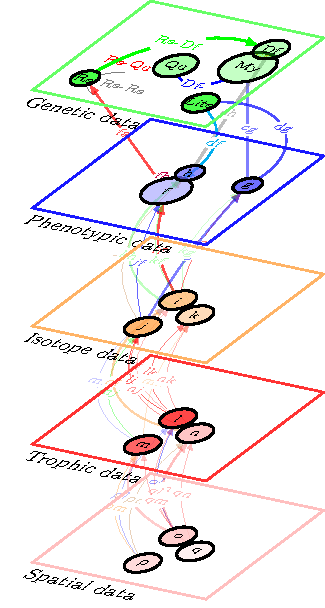
\includegraphics[width=13cm,height=16cm]{Figure2Stickle.pdf}
\\
\caption{{\small Figure 2: Example of the Threespine Stickleback multidimensional individual based database containing genetic, phenotypic, isotope, trophic and spatial data for around 1k individuals. This data is essentially QTL mapping (genetic data), morphological metrics of traits (phenotypic data), isotope and diet data and the spatial location (i.e., habitat type data).}}
\vspace{2 in}
\label{Figure 1}
\end{center}
\vspace{-4 in}

=======
>>>>>>> 9bd86e7a971d845b186e97178ddabf79dab974a8
\section*{4.2 Data sources}

We will combine animations, data mining for pattern inference (Box 1) and process-based
modeling (Box 2) to tangle genetic, phenotypic, ecological and spatial data. The following
are the available datasets:

Projet Lac database
Fish communities from the majority of lakes of Switzerland
Webpage: https://www.eawag.ch/en/department/fishec/projects/projet-lac/
The database contains approx. 60k fish individuals, 40k morphometrics and 8k sampling
actions each containing spatial coordinates, morphological traits, species abundances,
habitats and DNA data.

Whitefish community database
Whitefish community from the majority of lakes of North Alps.
The database contains more than 2k fish individuals. Sampling locations, morphological,
<<<<<<< HEAD
ecological and microsatellite data is available in the\\
=======
ecological and microsatellite data is available in the
>>>>>>> 9bd86e7a971d845b186e97178ddabf79dab974a8
Dryad database https://doi.org/10.5061/dryad.k183ft7

Threespine Stickleback database
The Threespine stickleback fish database contains genetic, isotope, diet, morphometric,
ecological and spatial data for around 1k individuals.
Hosting these datasets in the SDSC platform might allow us to
1. Featuring animations of the Fish collection part of the FishEc database in a future
permanent exhibition hosted by the Natural History Museum in Bern. The animations will
hightlight the interactions from genes to landscapes integrating genetic, phenotypic,
ecological and spatial data (see M1 and M2 below). Please check
https://www.nmbe.ch/de/unser-angebot/unser-angebot/fuer-forschende/wirbeltiere
section Ichthyologie with Projet Lac being one of the projects contributing the most to
the current FishEc database and https://www.nmbe.ch/de/museum/aktuelles/monster-im-
saft for the status of this permanent exhibition.
2. Inferring patterns of interdependence throughout new uploads of source data (M3 and
Box 1).
3. Analyzing process-based models to explore biodiversity dynamics scenarios with the
aim to infer the processes that best reproduce the empirical patterns observed in the
databases (M4 and Box 2).

\section*{4.3 Work Packages, Milestones and Deliverables}

This project will strengthen the feedback between data-scientists and the community of
scientists working with networks in ecology and evolution. This fusion will produce two
methods packages and two scientific papers. Below we describe the timeline describing the
milestones, the deliverables and the timing to release the packages in public repositories (Table
1).

<<<<<<< HEAD
CREATE TABLE LATEX

=======
>>>>>>> 9bd86e7a971d845b186e97178ddabf79dab974a8
Work packages
WP1: Data visualization (Lead: SDSC, contribution data: GENOM, ECOSYS, and BIOD)
WP2: Web spidering for source data and data integration (Lead: SDSC, contribution: MAIN
and BIOD)
WP3: Data mining (Lead: SDSC and MAIN, contribution: CSYS)
WP4: Process-based modeling (Lead: SDSC, MAIN and CSYS)

<<<<<<< HEAD
FIGURE MILESTONES

=======
>>>>>>> 9bd86e7a971d845b186e97178ddabf79dab974a8
Milestones
- M1.1: Uploading source data to Renga Platform
- M1.2: Visualization and animations of the source data as interdependent networks.
- M2.1: Web spidering to assist in the search of databases of the missing source data
- M2.2: Animation package of the Fish collection part of the FishEc database in the
permanent exhibition hosted by the Natural History Museum in Bern
- M3.1: Implementation of methods for inferring patterns in interdependent networks
(Box 1)
- M3.2: Efficient code implementation for inferring the interdependence among
networks
- M4.1: Implementing, debugging, running and analyzing the meta-ecosystem eco-
evolutionary network modeling scenarios (Box 2)
- M4.2: Analyzing the meta-ecosystem eco-evolutionary network modeling scenarios
parametrized using the inference patterns obtained in M3

%Table
Partner
WP
Year and Quarter
P
2019
L P
P
1
2 SDSC
SDSC GENOM
MAIN 3 SDSC MAIN CSYS M3.1
4 MAIN SDSC CSYS M4.1
1
ECOSYS BIOD M1.1
BIOD
2
M2.1
3
M1.2
4
M2.2
1
2020
2
3
4
D1
M3.2
D2 D3
M4.2 D4

Table 1


Deliverables
D1: Data visualization package to gain insights of the interactions across biological
networks from genes to metaecosystems.
The package will be used as highlights in the permanent exhibition of the natural
history museum in Bern. We will produce a public github repository and a
reproducible research document in Jupyter and Renga.
D2: Data mining and inference patterns and processes in interdependent networks
We will produce the inference package in interdependent networks. The package will
be uploaded and maintained in a github public repository. Together with the inference
package, we will produce a reproducible research document in Jupyter and Renga.
D3: Scientific paper focusing on inference patterns in interdependent networks
We will aim to a top general scientific journal. A reproducible research document
will be developed in github, Jupyter and Renga.
D4: Scientific paper focusing on process-based methods in interdependent networks
We will aim to a top general scientific journal. A reproducible research document
will be developed in github, Jupyter and Renga.

\section*{5. Requested Resources}

\section*{5.1 Staff}

\section*{5.1.1 Data science expertise}
A two years data scientist from the SDSC will be required to guarantee the accomplishment of
the word packages WP1 to WP4, and the deliverables D1 to D4
<<<<<<< HEAD
(see Requested resources and contributed resources below). The following are the key contributions for each stage of the project:

1. WP1: Software development to complement/improve the existing visualization and
animations tools for multilayer networks. Many libraries are rapidly emerging to integrate,
analyze, and visualize patterns in multilayer networks 123, yet add-hoc implementations in the
=======
(see
SDSC_full_proposal_requested_resources_Melian_2018.xlsx and contributed resources
below). The following are the key contributions for each stage of the project:
1. WP1: Software development to complement/improve the existing visualization and
animations tools for multilayer networks. Many libraries are rapidly emerging to integrate,
analyze, and visualize patterns in multilayer networks 123 , yet add-hoc implementations in the
>>>>>>> 9bd86e7a971d845b186e97178ddabf79dab974a8
existing tools or the development of new ones will be required to gain insights of the features
of interacting biological networks.
2. WP2: Machine Learning techniques and web spidering to assist in the search of databases to
improve data integration among genetic, phenotypic, ecological and spatial data.
3. WP3: Efficient code implementation to overcome the computational challenges of inferring
patterns of interactions connecting two or more networks across the webs of life (Figure 1 and
Box 1).
4. WP4: Analysis and debugging of the process-based modeling scenarios taking advantage of
the inference patterns obtained in WP3 to decipher the mechanisms explaining the observed
patterns in the integrated datasets (Box 2).
5.2. Compute and storage resources
5.2.1. Summary
We will need data storage and computing resources for running the visualizations, and the
simulations using the data-driven inference of patterns and processes. The following are the
working packages requiring computing and storage resources:
CSWP1: Running the visualizations for a small dataset containing 5-10k individuals with
genetic, phenotypic, ecological and spatial data. We would require to scale the visualization for
this subset to a much larger dataset containing approximately 60k fish individuals, 40k
morphometric measurements, and 8k sampling actions each containing spatial coordinates,
morphological traits, abundances, habitats and DNA data. We expect the need of
approximately
4
GPU
during
6
months
(see
SDSC_full_proposal_requested_resources_Melian_2018.xlsx) to run the visualizations and the
animations using the small and the large dataset and approx. 40 GPU servers RAM during a
total period of 8 months.



CSWP3: Implementing Gibbs sampling to fit the interaction coefficients for the interactions
within and between the genetic, phenotypic, ecological and spatial data (Box 1). Our estimated
need for CPU (cores) is of 35 for a 8 months period.
We expect to be working with the following data size:
1) Data containing 5-10k individuals each containing a 20x20 gene interaction matrix and a
40x40 phenotypic interaction matrix. The spatial data contains 0.1k-0.5k sites each containing
between 1 and 10 habitats. Each individual has coordinates within a habitat.
2) Data containing 50k individuals each containing a 40x40 gene interaction matrix and a
80x80 phenotypic interaction matrix. The spatial data contains 0.5k-1k sites each containing
between 1 and 10 habitats.
CSWP4: Implementing methods to fit process-based models to the empirical patterns (Box 2).
We will be working with matrices as described in CSWP3.

\section*{5.2.2 Software packages}

The following is the list of packages and skills to accomplish the deliverables D1 to D4:
1. Main skill: Spark GraphX to combine visualization, exploratory analysis and computation of
metrics to infer network patterns crossing two or more networks.
Additional skills: Implementation of packages in python (pymnet), java (gephi), and/or
octave/julia (muxviz) languages.
2. Main skill: Javascript/Jquery to enrich the data sources proposed to be analyzed with
external databases.
Additional skills: Implementation of codes in python, Ruby or others to search databases.
3. Main skill: TensorFlow. We have been working at a very preliminary stage with a julia
wrapper for TensorFlow 4 and we are open to learn from other packages to implement the
methods required in this proposal to make them more efficient and robust.
Additional skills: Hidden random Markov fields models or Bayesian methods to efficiently
compute and/or reconstruct interaction networks using genetic, phenotypic, ecological and
spatial data.

\section*{6. Contributed resources}
<<<<<<< HEAD
Dr. Victor Eguiluz, team CSYS, will join as a senior scientist during the spring 2019 to work in
the work packages WP3 (Data mining and inference) and WP4 (Process-based modeling). The
main task of Dr. Eguiluz will focus on (Table 2):
=======
Dr. Victor Egu�luz, team CSYS, will join as a senior scientist during the spring 2019 to work in
the work packages WP3 (Data mining and inference) and WP4 (Process-based modeling). The
main task of Dr. Egu�luz will focus on (Table 2):
>>>>>>> 9bd86e7a971d845b186e97178ddabf79dab974a8
1. Team up with the scientific staff of the SDSC to gain visualization insights of the ecological
and evolutionary processes underlying the data sources provided represented as multilayer
networks.
2. Implementing, debugging, running and analyzing the proposed meta-ecosystem eco-
evolutionary network modeling scenarios (Boxes 1 and 2).
3. Implementing linear algebra techniques to contrast the stability-diversity properties of
multilayer networks between scenarios driven by the empirical patterns and theoretical
scenarios using null or neutral models.
4. Drafting scientific paper focusing on inference patterns in interdependent networks
(Deliverables D2 and D3)
Table 1 shows the contributed resources from the staff. Please see the
SDSC_full_proposal_requested_resources_Melian_2018.xlsx document for a view of the total
contributed staff.
Table 2
CSYS Resource Type
(Researcher)
Dr. Victor Egu�luz Duration
Description of Role in the project
(in months)
100%
Drafting and implementing algorithms to
4 months
infer patterns and processes in
interdependent networks (WP3 and WP4).
Drafting scientific paper focusing on
pattern inference methods in
interdependent networks (deliverable D3)
MAIN Dr. Carlos Meli�n 30%
24 months
GENOM Dr. Philine Feulner
Partner
ECOSYS
BIOD
20%
2 months
Dr. Blake Matthews 20%
2 months
Prof. Ole Seehausen 10%
2 months
Teaming up with SDSC staff and Dr.
Egu�luz to develop pattern and process-
based inference packages (Deliverables D1
and D2 with SDSC and work packages
WP3 and WP4 with SDSC and Dr.
Egu�luz). Drafting scientific paper
focusing on process-based methods in
interdependent networks (deliverable D4)
Supervising accuracy of the genetic data
included in the FishEc dataset (WP1).
Drafting scientific papers focusing on
pattern inference and process-based
methods in interdependent networks
(deliverables D3 and D4)
Supervising accuracy of the genetic and
morphological data in the FishEc dataset
(WP1).
Supervision of the visualization package
(D1) and organization of the permanent
exhibition of the natural history museum in
Bern. Drafting scientific papers focusing
on pattern inference and process-based
methods in interdependent networks
(deliverables D3 and D4)

\newpage
\bibliographystyle{unsrtnat}
%\bibliographystyle{tree.bst}
\bibliography{space.bib}
\end{document}